\setcounter{section}{0}
\setcounter{viduii}{0}
	\viduii{2}{Tìm độ lớn hợp lực $\vec F$ của hai lực đồng quy $\vec{F}_1$ và $\vec{F}_2$ trong các trường hợp sau, nếu biết độ lớn $F_1=\SI{30}{N}$, $F_2=\SI{40}{N}$, góc giữa $\vec{F}_1$ và $\vec{F}_2$ là:
	\begin{enumerate}[label=\alph*.]
		\item $\alpha =0^\circ$.
		\item $\alpha =60^\circ$.
		\item $\alpha =90^\circ$.
		\item $\alpha =180^\circ$.
	\end{enumerate}
}
{	\begin{center}
		\textbf{Hướng dẫn giải}
	\end{center}
	
	\begin{enumerate}[label=\alph*.]
		\item Góc hợp bởi $\vec{F}_1$ và $\vec{F}_2$ là $\alpha =0^\circ$, tức là  $\vec{F}_1$ cùng chiều $\vec{F}_2.$
		
		Do đó, độ lớn $F=F_1+F_2= 70\, \si{\newton}$.
		\item Góc hợp bởi $\vec{F}_1$ và $\vec{F}_2$ là $\alpha =60^\circ.$
		
		Do đó, độ lớn $F=\sqrt{F_1^2+F_2^2+2F_1F_2\cos \alpha }= 10\sqrt{37}\,\si{\newton}$.
		\item Góc hợp bởi $\vec{F}_1$ và $\vec{F}_2$ là $\alpha =90^\circ$, tức là  $\vec{F}_1$ vuông góc $\vec{F}_2.$
		
		Do đó, độ lớn $F=\sqrt{F_1^2+F_2^2}=50\, \si{\newton}$.
		\item Góc hợp bởi $\vec{F}_1$ và $\vec{F}_2$ là $\alpha =180^\circ$, tức là  $\vec{F}_1$ ngược chiều $\vec{F}_2.$
		
		Do đó, độ lớn $F=|F_1-F_2|= 10\si{\newton}$.
	\end{enumerate}
	
}
	\viduii{2}{Một chất điểm chịu tác dụng đồng thời của hai lực thành phần vuông góc với nhau có độ lớn lần lượt là $F_1 = \SI{15}{N}$ và $F_2$. Biết hợp lực trên có độ lớn là $\SI{25}{N}$. Giá trị của $F_2$ là
	\begin{mcq}(4)
		\item $\SI{10}{N}$.
		\item $\SI{20}{N}$.
		\item $\SI{30}{N}$.
		\item $\SI{40}{N}$.
	\end{mcq}
}
{	\begin{center}
		\textbf{Hướng dẫn giải}
	\end{center}
	
	Nếu $\vec{F}_1$ vuông góc $\vec{F}_2$ thì về độ lớn: 
	
	$$F=\sqrt{F_1^2+F_2^2}$$
	
	Suy ra $F_2$: 
	
	$$F_2 = \sqrt {F^2 - F_1^2} = \SI{20}{N}.$$
	
	\textbf{Đáp án: B}.
}
\section{Trắc nghiệm}
\begin{enumerate}[label=\bfseries Câu \arabic*:]
	
	\item \mkstar{1}
	
	{ Muốn cho một chất điểm cân bằng thì hợp lực của các lực tác dụng lên nó phải	
		\begin{mcq}(2)
			\item không đổi.
			\item thay đổi.
			\item bằng 0.
			\item khác 0.
		\end{mcq}
	}
	
	\hideall{
		\textbf{Đáp án: C.}
		
		Muốn cho một chất điểm cân bằng thì hợp lực của các lực tác dụng lên nó phải bằng 0.
	}
	\item \mkstar{1}
	
	{ Độ lớn của hợp lực $\vec{F}$ hai lực $\vec{F}_1$ và $\vec{F}_2$  đồng qui hợp với nhau góc $\alpha$ là
		\begin{mcq}(2)
			\item $\sqrt{F_1^2+F_2^2-2F_1F_2\cos \alpha}$.
			\item $\sqrt{F_1^2+F_2^2+2F_1F_2\cos \alpha}$.
			\item $\sqrt{F_1^2+F_2^2-F_1F_2\cos \alpha}$.
			\item $\sqrt{F_1^2+F_2^2+F_1F_2\cos \alpha}$.
		\end{mcq}
	}
	\hideall{	
		\textbf{Đáp án: B.}
		
		Ta có: $$F = \sqrt{F_1^2+F_2^2+2F_1F_2\cos \alpha}.$$
	}
	\item \mkstar{1}
	
	{ Tổng hợp lực là 
		\begin{mcq}
			\item thay thế một lực bằng các lực có tác dụng giống hệt như các lực ấy.
			\item thay thế các lực tác dụng đồng thời vào cùng một vật bằng một lực có tác dụng giống hệt như các lực ấy.
			\item thay thế các lực tác dụng đồng thời hai vật bằng một lực có tác dụng giống hệt như các lực ấy.
			\item thay thế hai lực bằng ba lực có tác dụng giống hệt như các lực ấy.
		\end{mcq}
	}
	\hideall{		\textbf{Đáp án: B.}
		
		Tổng hợp lực là thay thế các lực tác dụng đồng thời vào cùng một vật bằng một lực có tác dụng giống hệt như các lực ấy.
	}
	\item \mkstar{2}
	
	{ Một chất điểm đứng yên dưới tác dụng của $3$ lực có độ lớn bằng nhau. Kết luận nào sau đây là đúng?
		\begin{mcq}
			\item 	Có 2 lực cùng giá, ngược chiều nhau.
			\item  Ba lực có giá cùng nằm trong 1 mặt phẳng, chúng lần lượt hợp với nhau những góc $120^\circ$.
			\item Ba lực có giá cùng nằm trong một mặt phẳng, trong đó $2$ lực có giá vuông góc nhau.
			\item Cả A, B, C đều sai.
			
		\end{mcq}
	}
	\hideall{		\textbf{Đáp án: B.}	
		
		Một chất điểm đứng yên dưới tác dụng của $3$ lực có độ lớn bằng nhau thì ba lực có giá cùng nằm trong 1 mặt phẳng, chúng lần lượt hợp với nhau những góc $120^\circ$.
		
	}
	\item \mkstar{2}
	
	{ Tác dụng vào một vật đồng thời hai lực $\vec{F_1}$  và $\vec{F_2}$ trong đó độ lớn $F_1 = 30\ \text{N}$ và $F_1 = 40\ \text{N}$. Nhận xét nào sau đây là đúng?
		\begin{mcq}
			\item Hợp lực tác dụng lên vật có độ lớn $70\ \text{N}$.
			\item Hợp lực tác dụng lên vật có độ lớn $10\ \text{N}$.
			\item Hợp lực tác dụng lên vật có độ lớn $50\ \text{N}$.
			\item Chưa đủ cơ sở để kết luận.
		\end{mcq}
	}
	\hideall{		\textbf{Đáp án: D.}
		
		Vì chưa biết $\alpha$ hợp bởi hai lực  $\vec{F_1}$  và $\vec{F_2}$ nên ta chưa đủ cơ sở để kết luận.
	}
	
	
	\item \mkstar{2}
	
	{ Điều nào sau đây là \textbf{sai} khi nói về đặc điểm của hai lực cân bằng? 
		
		\begin{mcq}(2)
			\item Hai lực có cùng giá.
			\item Hai lực đặt vào hai vật khác nhau.
			\item Hai lực ngược chiều nhau.
			\item Hai lực có cùng độ lớn.
		\end{mcq}
	}
	\hideall{		\textbf{Đáp án: B.}
		
		Hai lực cân bằng đặt vào cùng một vật.
		
	}
	
	\item \mkstar{2}
	
	{ Hai lực có giá đồng quy có độ lớn $F_1=F_2=10\ N$, có $(\overrightarrow {F_1}, \overrightarrow {F_2})=60^\circ$. Hợp lực của hai lực này có độ lớn là
		\begin{mcq}(4)
			\item $\text{17,3}\, \si{\newton}$.
			\item $\text{20}\, \si{\newton}$.
			\item $\text{14,1}\, \si{\newton}$.
			\item $\text{10}\, \si{\newton}$.
		\end{mcq}
		
	}
	\hideall{		\textbf{Đáp án: A.}
		
		Áp dụng công thức $$F^2=F_1^2+F_2^2+2F_1F_2.\cos(\overrightarrow {F_1}, \overrightarrow {F_2}) $$
		
		Thay số liệu vào, ta tìm được $$F=\text{17,3}\, \si{\newton}$$
	}
	\item \mkstar{3}
	
	{ Một chất điểm chịu tác dụng đồng thời của hai lực thành phần có độ lớn $F_1$ và $F_2$ thì hợp lực F của chúng luôn có độ lớn thỏa mãn hệ thức:
		\begin{mcq}(2)
			\item $F=F_1^2+F_2^2$.
			\item $F = F_1 + F_2$.
			\item $|F_1-F_2| \leq F \leq F_1 + F_2$.
			\item $F= \sqrt{F_1^2+F_2^2}$.
		\end{mcq}
		
	}
	\hideall{		\textbf{Đáp án: C.}
		
		Theo lý thuyết:	$$|F_1-F_2| \leq F \leq F_1 + F_2$$
		
		
	}
	\item \mkstar{3}
	
	{ Cho hai lực đồng quy có độ lớn bằng $12\ \text{N}$ và $16\ \text{N}$ hợp nhau một góc $\alpha$. Độ lớn và góc hợp bởi hai lực đó là 
		\begin{mcq}(2)
			\item $3\ \text{N}$ và $30^\circ$.
			\item $20\ \text{N}$ và $90^\circ$.
			\item $30\ \text{N}$ và $60^\circ$.
			\item $40\ \text{N}$ và $45^\circ$.
		\end{mcq}
	}
	\hideall{		\textbf{Đáp án: B.}
		
		Với $\alpha=90^\circ$
		
		Độ lớn và góc hợp bởi hai lực đó là 
		$$F=\sqrt{F_1^2+F_2^2}=20\ \text{N}.$$
		
		
	}
	
	\item \mkstar{4}
	
	{ Một thanh đồng chất nằm cân bằng ở tư thế nằm ngang bởi hai sợi dây buộc vào hai đầu của nó như hình vẽ. Lực căng dây có độ lớn $T_1=T_2=\SI{10}{\newton}$, góc $\theta=37^\circ$. Trọng lượng của thanh bằng
		\begin{center}
			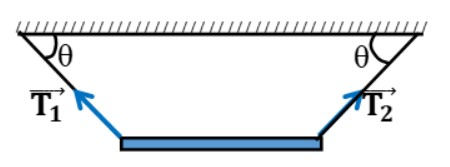
\includegraphics[scale=0.7]{../figs/VN10-2021-PH-TP011-5.jpg}
		\end{center}
		\begin{mcq}(4)
			\item $\SI{10}{\newton}$.
			\item $\SI{20}{\newton}$.
			\item $\SI{12}{\newton}$.
			\item $\SI{16}{\newton}$.
		\end{mcq}
		
		
	}
	\hideall{		\textbf{Đáp án: C.}
		
		Trọng lượng của thanh bằng
		$$P=mg=2T\sin\theta=\SI{12}{\newton}.$$
		
	}
\end{enumerate}



\hideall
{
	\begin{center}
		\textbf{BẢNG ĐÁP ÁN}
	\end{center}
	\begin{center}
		\begin{tabular}{|m{2.8em}|m{2.8em}|m{2.8em}|m{2.8em}|m{2.8em}|m{2.8em}|m{2.8em}|m{2.8em}|m{2.8em}|m{2.8em}|}
			\hline
			1.C  & 2.B  & 3.B  & 4.B  & 5.D  & 6.B  & 7.A  & 8.C  & 9.B  & 10.C  \\
			\hline
			
		\end{tabular}
	\end{center}
}
\section{Tự luận}
\begin{enumerate}[label=\bfseries Câu \arabic*:]
	\item \mkstar{1}
	
	{
		Phát biểu định nghĩa của lực và điều kiện cân bằng của một chất điểm.
	}
	
	\hideall{
		
		Lực là một đại lượng vec-tơ đặc trưng cho sự tác dụng của vật này vào vật khác mà kết quả là gây ra gia tốc cho vật hoặc làm cho vật bị biến dạng.
		
		Điều kiện cân bằng của một chất điểm: Tổng hợp lực tác dụng vào vật bằng 0.
	}
	\item \mkstar{2}
	
	{
		Cho hai lực đồng quy có độ lớn $F_1 = \SI{6}{N}$ và $F_2 = \SI{8}{N}$. Nếu hợp lực có độ lớn $F = \SI{10}{N}$ thì góc giữa hai lực $\vec F_1$ và $\vec F_2$ bằng bao nhiêu?
	}
	
	\hideall{
		
		Theo đề bài
		
		$$10^2 = 6^2 + 8^2.$$
		
		Hay
		
		$$F = \sqrt{F_1^2+F_2^2}.$$
		
		Suy ra:
		
		$\vec F_2$ vuông góc với $\vec F_1$
		
	}

	\item \mkstar{2}
	
	{ Một trái banh được tác dụng lực $\vec{F_1}$ bởi gió và $\vec{P}$ bởi trọng lực, hai lực này có giá vuông góc với nhau và độ lớn $F_1=P=\SI{10}{N}$. Hãy tính độ lớn của lực $\vec{F_3}$ là lực tổng hợp của hai lực trên.
		
	}
	\hideall{
		
		Do hai vectơ vuông góc nhau nên $$F_3= \sqrt{F_1^2+P^2}=10\sqrt{2}\, \textrm{N}$$
	}
	\item \mkstar{3}
	
	{Giả sử lực kéo của mỗi tàu kéo ở đầu bài đều có độ lớn $\SI{8000}{N}$ và góc giữa hai dây cáp bằng $30^\circ$. 
		\begin{enumerate}[label=\alph*)]
			\item Biểu diễn các lực kéo của mỗi tàu và hợp lực tác dụng vào tàu chở hàng.
			\item Tính độ lớn của hợp lực của hai lực kéo.
			\item Nếu góc giữa hai dây cáp bằng $90^\circ$ thì hợp lực của hai lực kéo có phương, chiều và độ lớn như thế nào?
		\end{enumerate}
		
	}
	
	\hideall{
		\begin{enumerate}[label=\alph*)]
			\item Biểu diễn các lực kéo của mỗi tàu và hợp lực tác dụng vào tàu chở hàng
			
		\begin{center}
			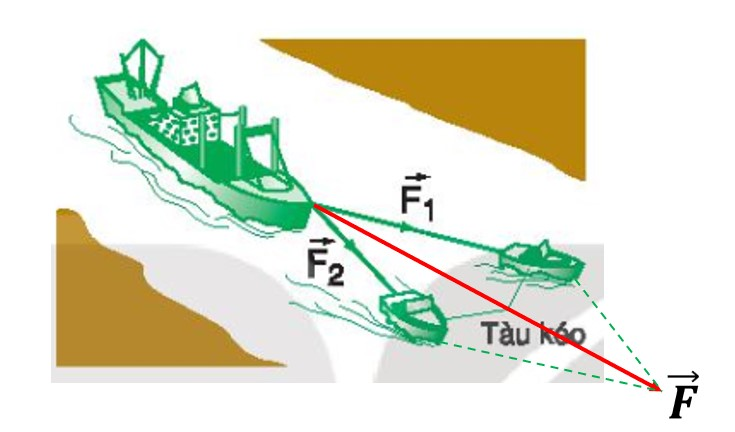
\includegraphics[scale=0.7]{../figs/VN10-2022-PH-TP015-4.jpg}
		\end{center}
	
			
			\item Độ lớn của hợp lực của hai lực kéo
			
			$$F = \sqrt{F_1^2 + F_2^2 - 2F_1F_2 \cos 30^\circ} = \SI{4160}{N}.$$
			
			\item Nếu góc giữa hai dây cáp bằng $90^\circ$ thì
			
			$$F = \sqrt{F_1^2+F_2^2} = \SI{11280}{N}.$$
			
			Hợp lực tạo với phương ngang 1 góc $45^\circ$.
		\end{enumerate}
		
	}
	\item \mkstar{2}
	
	{
		Quan sát quyển sách đang nằm yên trên mặt bàn.
		
		\begin{center}
			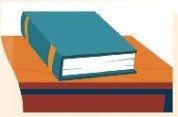
\includegraphics[scale=0.7]{../figs/VN10-2022-PH-TP015-5.jpg}
		\end{center}
		\begin{enumerate}[label=\alph*)]
			\item Những lực nào tác dụng lên quyển sách?
			\item Các lực này có cân bằng không? Vì sao?
		
		\end{enumerate}
	}
	
	\hideall{
		
		\begin{enumerate}[label=\alph*)]
			\item Những lực nào tác dụng lên quyển sách:
			
			- Trọng lực của Trái Đất.
			
			- Lực đỡ cửa mặt bàn.
			
			\item Các lực này cân bằng nhau vì quyển sách vẫn nằm im, không xê dịch.
			
		\end{enumerate}
	}
		\item \mkstar{3}
	
	{
	Một ô tô chịu một lực $F_1 = \SI{400}{N}$ hướng về phía trước và một lực $F_2 = \SI{300}{N}$ hướng về phía sau. Hỏi hợp lực tác dụng lên ô tô có độ lớn bằng bao nhiêu và hướng về phía nào?
	
	\begin{center}
		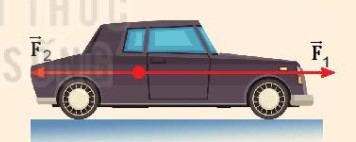
\includegraphics[scale=0.7]{../figs/VN10-2022-PH-TP015-1.jpg}
	\end{center}
	
	}
	
	\hideall{
		
		 Hợp lực tác dụng lên ô tô có độ lớn là
		 
		 $$F = F_1 - F_2 = 400-300 = \SI{100}{N}.$$
		 
		  Lực $F$ cùng hướng với lực $F_1$.
		
	}
	\item \mkstar{3}
	
	{
		Quan sát mỗi cặp tình huống ở hình.
		\begin{enumerate}[label=\alph*)]
			\item Tình huống nào có hợp lực khác 0?
			\item Mô tả sự thay đổi vận tốc (độ lớn, hướng) của mỗi vật trong hình, nếu có.
			
		\end{enumerate}
		
		\begin{center}
			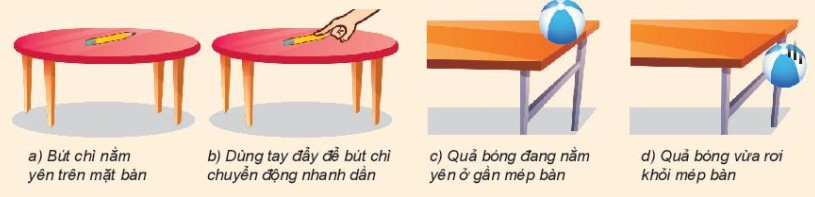
\includegraphics[scale=0.7]{../figs/VN10-2022-PH-TP015-2.jpg}
		\end{center}
		
	}
	
	\hideall{
		
		\begin{enumerate}[label=\alph*)]
			\item Cặp a và b: Hợp lực tác dụng lên bút trên bàn ở hình a là bằng không, hình b là khác không.
			
			Cặp c và d : Hợp lực tác dụng lên qủa bóng ở hình c là bằng không, hình d là khác 0
			\item Hình a và c thì bút và quả bóng sẽ nằm im một chỗ. 
			
			Hình b thì bút sẽ thay đổi vận tốc theo lực mà tay tác động vào, và hướng là cùng hướng với lực của tay. 
			
			Hình d thì quả bóng có vận tốc rơi càng lúc càng nhanh hơn do tác động của trọng lực, hướng xuống dưới.
			
		\end{enumerate}
		
	}
		\item \mkstar{3}
	
	{
		Một vật được giữ yên trên một mặt phẳng nghiêng nhẵn bởi một lò xo.
		\begin{center}
			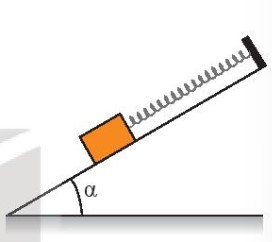
\includegraphics[scale=0.7]{../figs/VN10-2022-PH-TP015-3.jpg}
		\end{center}
	
			\begin{enumerate}[label=\alph*)]
			\item Có những lực nào tác dụng lên vật?
			\item Phân tích trọng lực tác dụng lên vật thành hai lực thành phần và nêu rõ tác dụng của hai lực này.
			
		\end{enumerate}
		
	
		
	}
	
	\hideall{
		
	\begin{enumerate}[label=\alph*)]
		\item Lực tác dụng lên vật:
		
		- Trọng lực $\vec P$.
		
		- Phản lực $\vec N$.
		
		- Lực kéo $\vec F$.
		
		- Lực đàn hồi của lò xo.
		
		\item 
		\begin{center}
			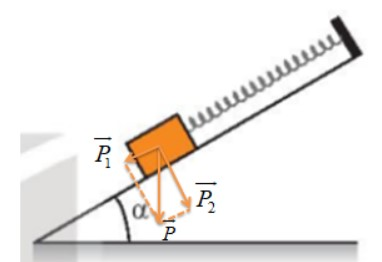
\includegraphics[scale=0.7]{../figs/VN10-2022-PH-TP015-6.jpg}
		\end{center}
		
		- Thành phần $\vec P_1$ có tác dụng kéo vật chuyển động xuống phía dưới.
		
		- Thành phần $\vec P_2$ có tác dụng giữ vật trên mặt phẳng nghiêng.
		
	\end{enumerate}
	
	}
	\item \mkstar{3}
	
	{ Chất điểm chịu tác dụng đồng thời của hai lực $\vec{F}_1$ và $\vec{F}_2$ có cùng độ lớn là $10\ \text{N}$. Góc giữa hai véctơ $\vec{F}_1$ và $\vec{F}_2$  bằng $30^\circ$. Tính độ lớn của hợp lực.
	}
	\hideall{
		
		Hai lực $\vec{F_1}$  và $\vec{F_2}$ có cùng độ lớn  hợp với nhau một góc $\alpha$. 
		
		Hợp lực của chúng có độ lớn là  $$F=2F_1\cos \left( \dfrac{\alpha}{2}\right)=\text{19,3}\ \text{N} $$
	}
	\item \mkstar{4}
	
	{ Một quả cầu đồng chất có khối lượng $\SI{4}{\kilogram}$ được treo vào tường thẳng đứng nhờ một sợi dây hợp với tường một góc $\alpha=30^\circ$. Bỏ qua ma sát ở chỗ tiếp xúc của quả cầu với tường. Lấy $g=\SI{9,8}{\meter/\second^2}$. Tính lực của tường tác dụng lên quả cầu.
		\begin{center}
			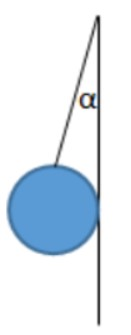
\includegraphics[scale=0.8]{../figs/VN10-2021-PH-TP011-3.jpg}
		\end{center}
	}
	\hideall{
		
		Các lực tác dụng lên quả cầu được biểu diễn như hình vẽ:
		\begin{center}
			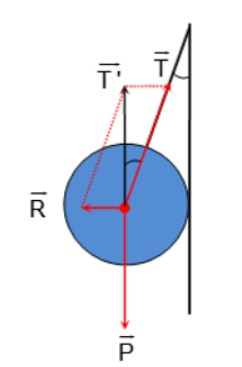
\includegraphics[scale=0.7]{../figs/VN10-2021-PH-TP011-4.jpg}
		\end{center}
		Điều kiện cân bằng của quả cầu là:
		$$\vec{R}+\vec{T}=\vec{T}'=-\vec{P}.$$
		Ta có:
		$$\tan\alpha=\dfrac{R}{P}\Rightarrow R=P\cdot \tan\alpha=\SI{22,6}{\newton}.$$
	}

\end{enumerate}